
%%%%%%%%%%%%%%%%%%%%%%%%%%%%%%%%%%%%%%%%%%%%%%%%%%%%%%%%%%%%%%%%%%%%%%%%%%%%%%%%%%
\begin{frame}[fragile]\frametitle{}
\begin{center}
{\Large  Stages Centered Around Large Language Models}

{\tiny (Ref: 5 stages of Generative AI project lifecycle - Abhinav Kimothi)}

\end{center}
\end{frame}

%%%%%%%%%%%%%%%%%%%%%%%%%%%%%%%%%%%%%%%%%%%%%%%%%%%%%%%%%%%
\begin{frame}[fragile]\frametitle{5 stages of Generative AI project lifecycle}


		\begin{center}
		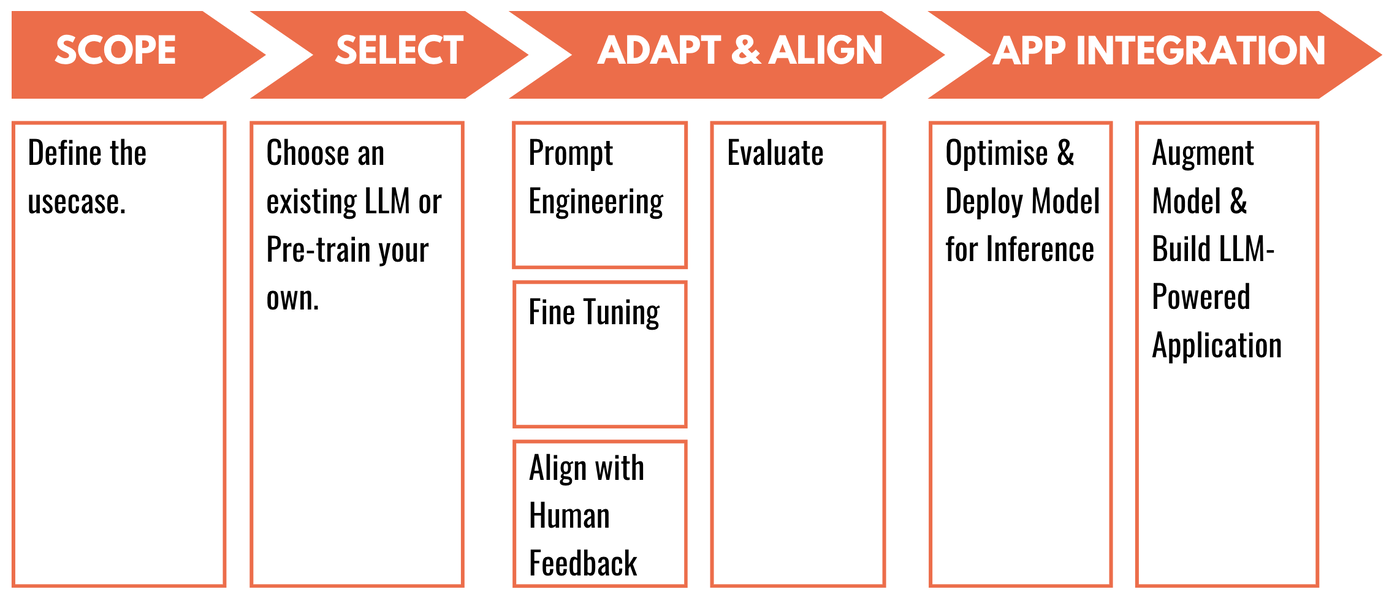
\includegraphics[width=\linewidth,keepaspectratio]{llm106}
		\end{center}

{\tiny (Ref: 5 stages of Generative AI project lifecycle - Abhinav  Kimothi)}

\end{frame}


%%%%%%%%%%%%%%%%%%%%%%%%%%%%%%%%%%%%%%%%%%%%%%%%%%%%%%%%%%%
\begin{frame}[fragile]\frametitle{Project LifeCycle}


		\begin{center}
		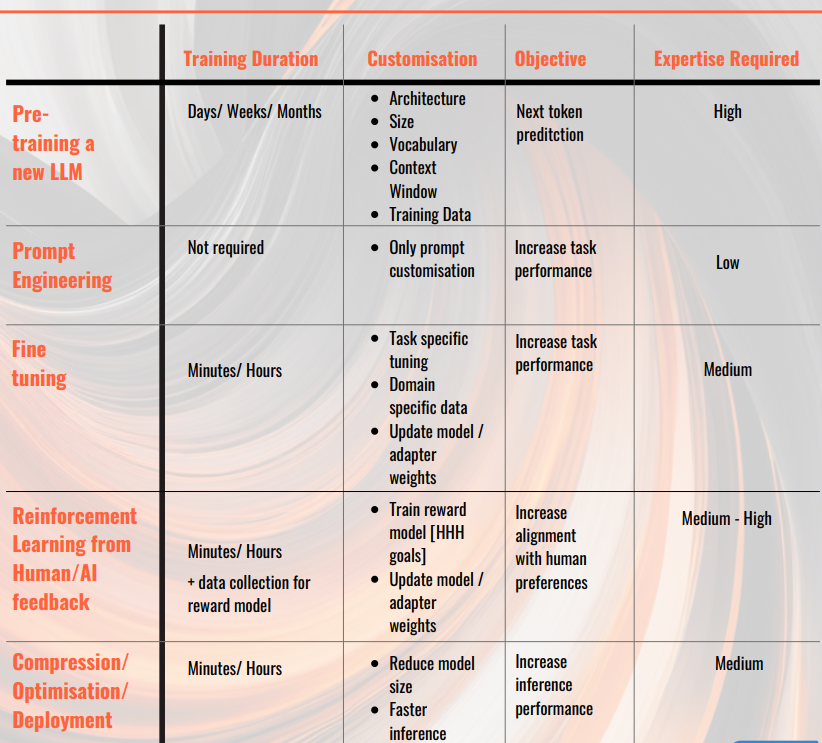
\includegraphics[width=\linewidth,keepaspectratio]{rag5}
		\end{center}

{\tiny (Ref: 5 stages of Generative AI project lifecycle - Abhinav  Kimothi)}

\end{frame}


%%%%%%%%%%%%%%%%%%%%%%%%%%%%%%%%%%%%%%%%%%%%%%%%%%%%%%%%%%%%%%%%%%%%%%%%%%%%%%%%%%
\begin{frame}[fragile]{Stage 1: Pre-training}
    \begin{itemize}
        \item Building an LLM from scratch (e.g., BERT, GPT4, Llama 2).
        \item Unsupervised Learning for text generation or next token prediction.
        \item Training involves billions of parameters on a large corpus.
        \item Compute-intensive phase lasting days or even months.
        \item Decisions on training corpus and transformer architecture are made.
        \item Result: Foundation Models for subsequent stages.
    \end{itemize}
\end{frame}

%%%%%%%%%%%%%%%%%%%%%%%%%%%%%%%%%%%%%%%%%%%%%%%%%%%%%%%%%%%%%%%%%%%%%%%%%%%%%%%%%%
\begin{frame}[fragile]{Stage 2: Prompt Engineering}
    \begin{itemize}
        \item Foundation model ready for text generation.
        \item Inference through prompt input without training.
        \item No modification of model weights during this phase.
        \item Examples given are in-context prompts.
        \item Objective: Improve performance on generated text.
    \end{itemize}
	
		\begin{center}
		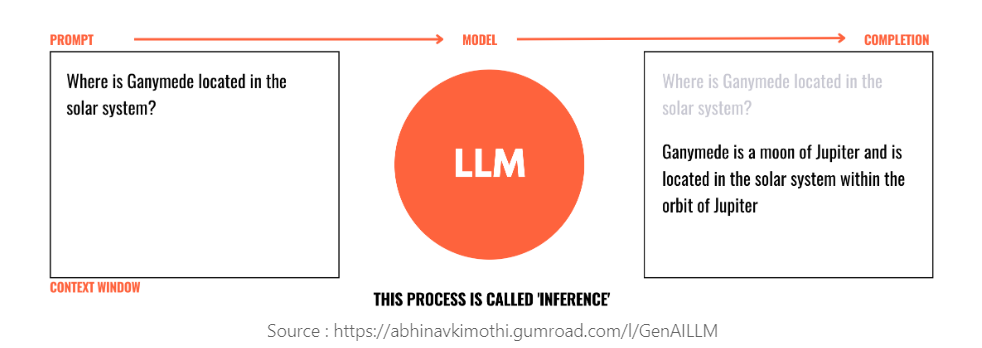
\includegraphics[width=\linewidth,keepaspectratio]{llm107}
		\end{center}	
\end{frame}

%%%%%%%%%%%%%%%%%%%%%%%%%%%%%%%%%%%%%%%%%%%%%%%%%%%%%%%%%%%%%%%%%%%%%%%%%%%%%%%%%%
\begin{frame}[fragile]{Stage 3: Fine-tuning}
    \begin{itemize}
        \item Critical phase for task-specific performance.
        \item Supervised Learning task using prompts and completions.
        \item Requires significant memory, comparable to pre-training.
        \item Updates weights of the foundation model.
        \item Parameter Efficient Fine Tuning (PEFT) reduces memory requirements while maintaining performance.
    \end{itemize}
	
		\begin{center}
		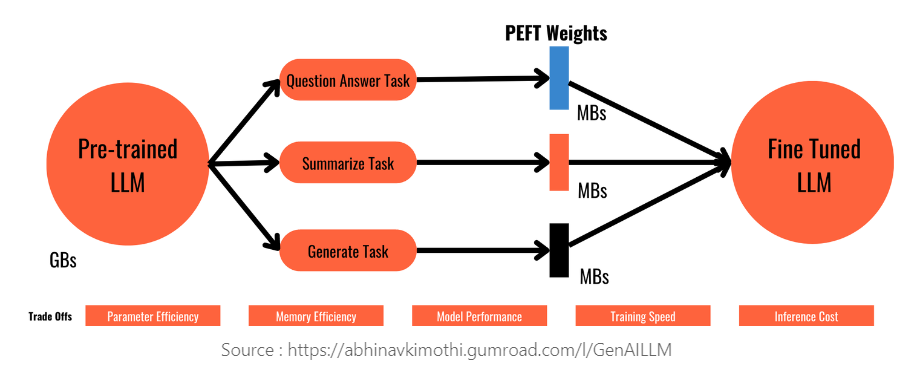
\includegraphics[width=\linewidth,keepaspectratio]{llm108}
		\end{center}	
\end{frame}

%%%%%%%%%%%%%%%%%%%%%%%%%%%%%%%%%%%%%%%%%%%%%%%%%%%%%%%%%%%%%%%%%%%%%%%%%%%%%%%%%%
\begin{frame}[fragile]{Stage 4: Reinforcement Learning from Human/AI Feedback}
    \begin{itemize}
        \item RLHF or RLAIF pivotal for LLM acceptance.
        \item Aligns LLM to human values (Helpfulness, Harmlessness, Honesty) using rewards.
        \item Initial rewards provided by humans; rewards model is generated.
        \item Constitutional AI principles used to scale human feedback.
        \item Result: LLM aligned with human values.
    \end{itemize}
	
		\begin{center}
		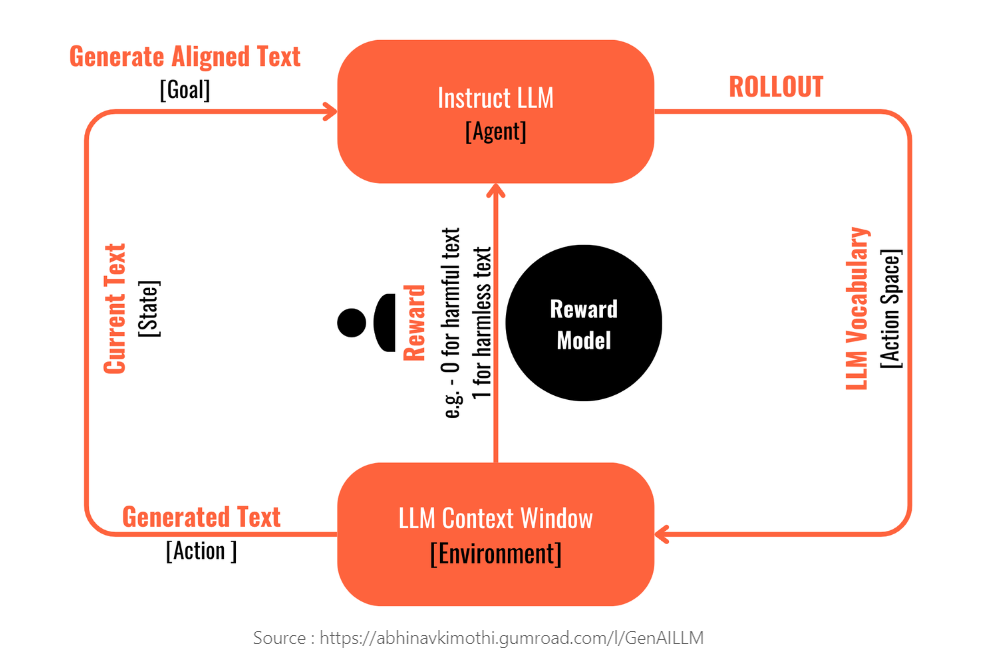
\includegraphics[width=\linewidth,keepaspectratio]{llm109}
		\end{center}	
\end{frame}

%%%%%%%%%%%%%%%%%%%%%%%%%%%%%%%%%%%%%%%%%%%%%%%%%%%%%%%%%%%%%%%%%%%%%%%%%%%%%%%%%%
\begin{frame}[fragile]{Stage 5: Compression, Optimisation, and Deployment}
    \begin{itemize}
        \item Final stage for application usage.
        \item Model optimized for faster inference and reduced memory.
        \item Sometimes, a smaller LLM derived from the original is used in production.
    \end{itemize}
	
		\begin{center}
		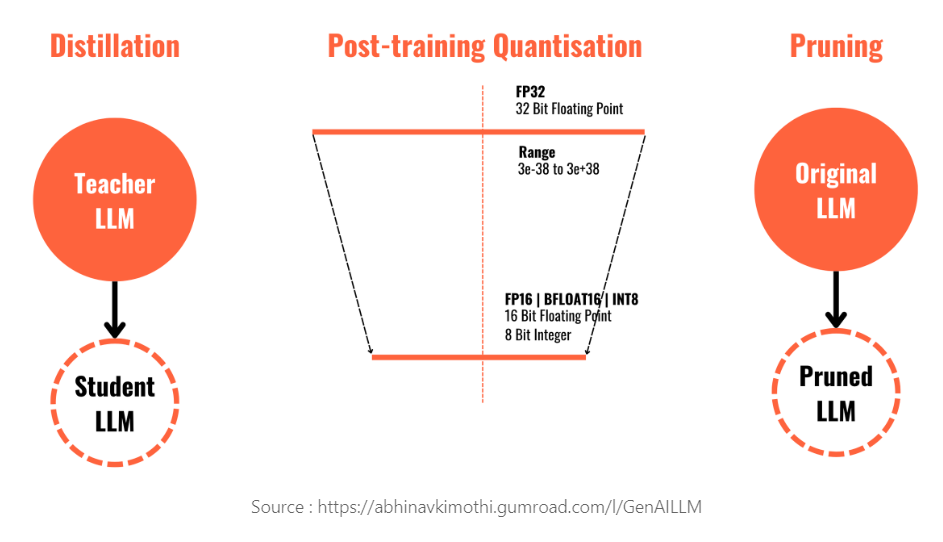
\includegraphics[width=\linewidth,keepaspectratio]{llm110}
		\end{center}		
\end{frame}


%%%%%%%%%%%%%%%%%%%%%%%%%%%%%%%%%%%%%%%%%%%%%%%%%%%%%%%%%%%%%%%%%%%%%%%%%%%%%%%%%%
\begin{frame}[fragile]\frametitle{}
\begin{center}
{\Large LLM in Production}

{\tiny (Ref: MLOps.community channel on Youtube)}

\end{center}
\end{frame}



%%%%%%%%%%%%%%%%%%%%%%%%%%%%%%%%%%%%%%%%%%%%%%%%%%%%%%%%%%%
\begin{frame}[fragile]\frametitle{Compare before use}

\begin{center}
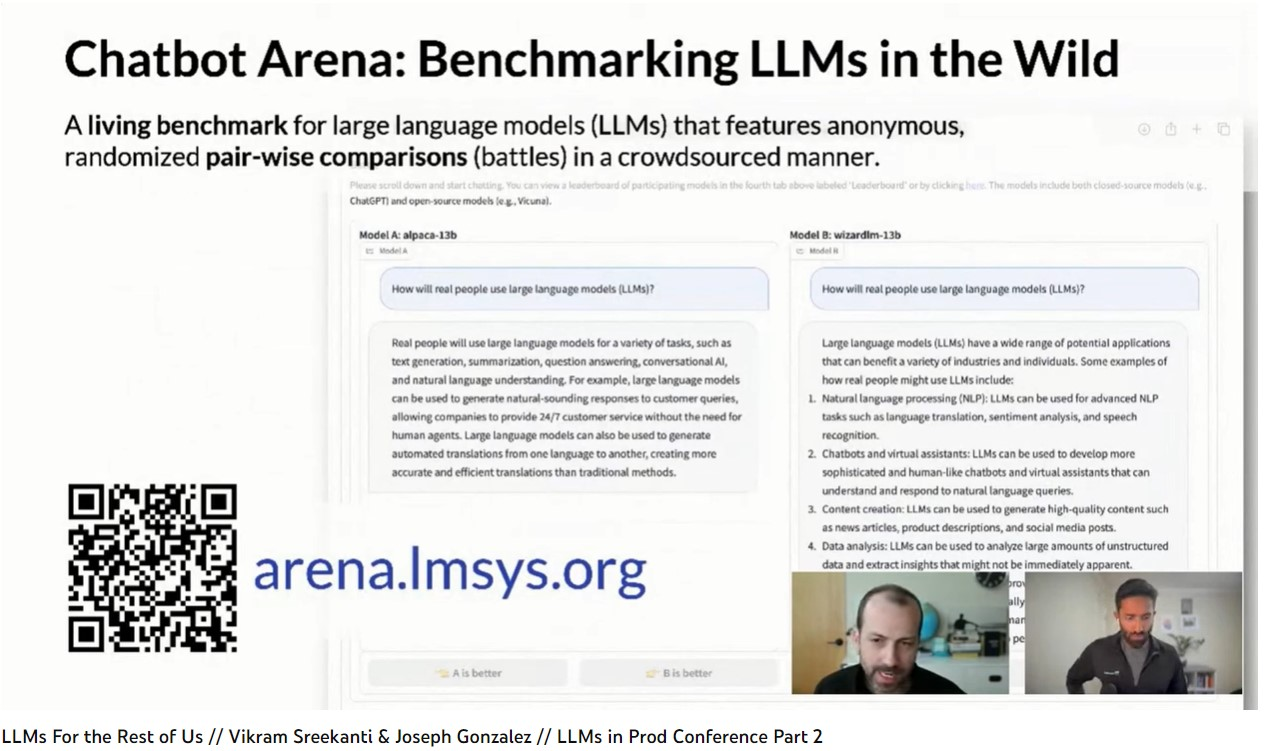
\includegraphics[width=\linewidth,keepaspectratio]{llm57}
\end{center}
\end{frame}

%%%%%%%%%%%%%%%%%%%%%%%%%%%%%%%%%%%%%%%%%%%%%%%%%%%%%%%%%%%
\begin{frame}[fragile]\frametitle{Missing Link}
\begin{columns}
    \begin{column}[T]{0.5\linewidth}
		\begin{itemize}
		\item Good models are hosted ones, so you tend to build own (foundation) model, do you really need it? Use largest that you can afford/use.
		\item Use your own data via Vector Databases
		\item Exhausting prompt engineering, chaining, orchestration frameworks.
		\item Be specific and not expect that models will do everything.
		\item Have good data quality and governance and also good Validation, tracing and logging.
		\end{itemize}	
    \end{column}
    \begin{column}[T]{0.5\linewidth}
		\begin{center}
			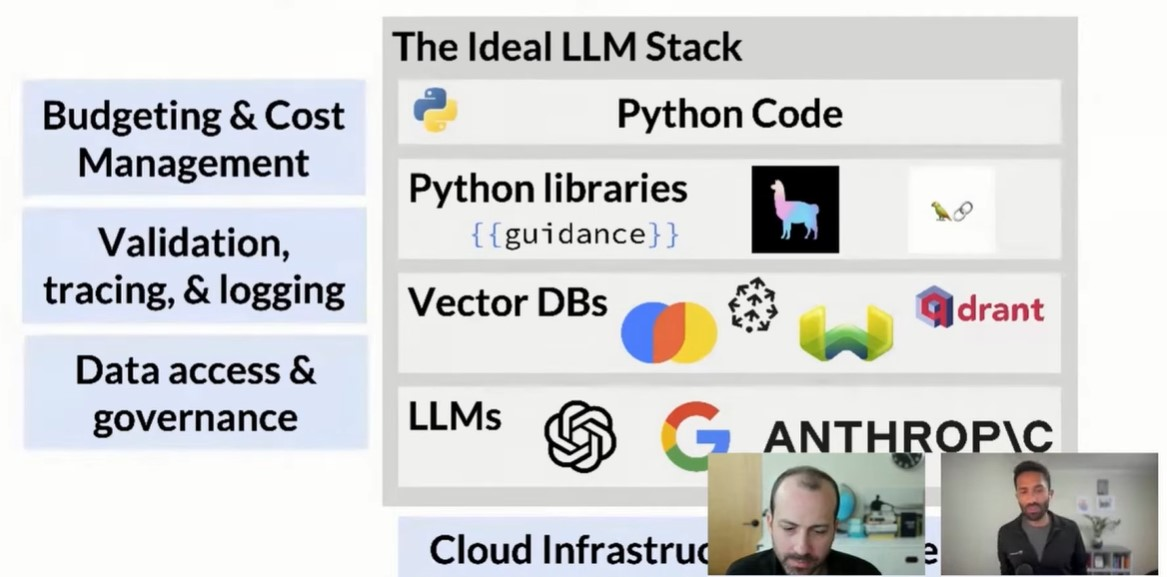
\includegraphics[width=\linewidth,keepaspectratio]{llm58}
		\end{center}
	\end{column}
  \end{columns}
\end{frame}


%%%%%%%%%%%%%%%%%%%%%%%%%%%%%%%%%%%%%%%%%%%%%%%%%%%%%%%%%%%
\begin{frame}[fragile]\frametitle{Customizing Solutions}

\begin{itemize}
\item Fine tuning: few shots, whole model
\item Hand crafted prompts
\item Optimization
	\begin{itemize}
	\item Programmatic prompt generation (human readable)
	\item AutoPrompt (Gradient based searches), not human readable
	\item Continuous: P-tuning, Prefix-tuning
	\end{itemize}
\item RLHF (Reinforcement Learning with Human Feedback)
\end{itemize}	

Which one is most appropriate? What about platforms which provide customization?
\end{frame}


%%%%%%%%%%%%%%%%%%%%%%%%%%%%%%%%%%%%%%%%%%%%%%%%%%%%%%%%%%%
\begin{frame}[fragile]\frametitle{Evaluation}

\begin{itemize}
\item `Hero` use cases ( say smoke test, must work)
\item White box testing
\item Edge cases, missing conflicting data
\item User feedback, bugs
\item Out of scope functionality, graceful denial.
\end{itemize}

{\tiny (Ref: Combining LLMs with Knowledge Bases to Prevent Hallucinations - Scott Mackie - LLMs in Prod Con 2 )}

\end{frame}

%%%%%%%%%%%%%%%%%%%%%%%%%%%%%%%%%%%%%%%%%%%%%%%%%%%%%%%%%%%
\begin{frame}[fragile]\frametitle{How to Evaluate}

\begin{itemize}
\item We don't have test-train distribution used during training, as we did not do the trainin itself. So there is always a DRIFT.
\item Evaluation is qualitative than quantitative.
\item Trained on ALL subjects but being used for ONE/TWO domains, hard to measure then.
\end{itemize}

\begin{center}
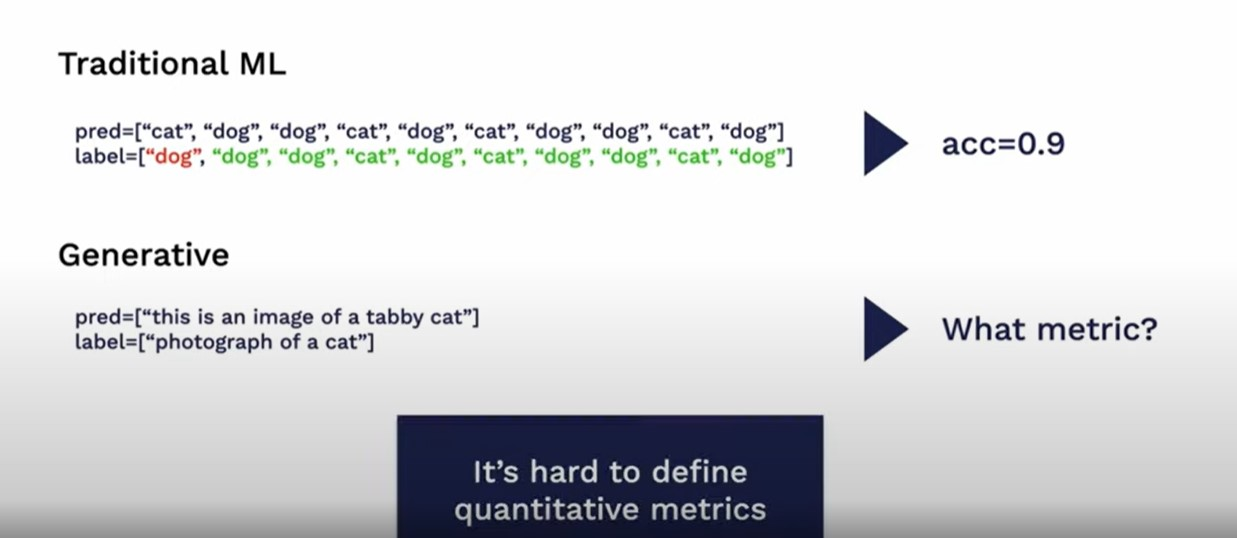
\includegraphics[width=0.6\linewidth,keepaspectratio]{llm68}
\end{center}		


{\tiny (Ref: Evaluating LLM-based Applications // Josh Tobin // LLMs in Prod Conference Part 2 )}

\end{frame}

%%%%%%%%%%%%%%%%%%%%%%%%%%%%%%%%%%%%%%%%%%%%%%%%%%%%%%%%%%%
\begin{frame}[fragile]\frametitle{How much it costs to Evaluate}

\begin{itemize}
\item We don't have test-train distribution used during training, as we did not do the trainin itself. So there is always a DRIFT.
\item Evaluation is qualitative than quantitative.
\item Trained on ALL subjects but being used for ONE/TWO domains, hard to measure then.
\end{itemize}

\begin{center}
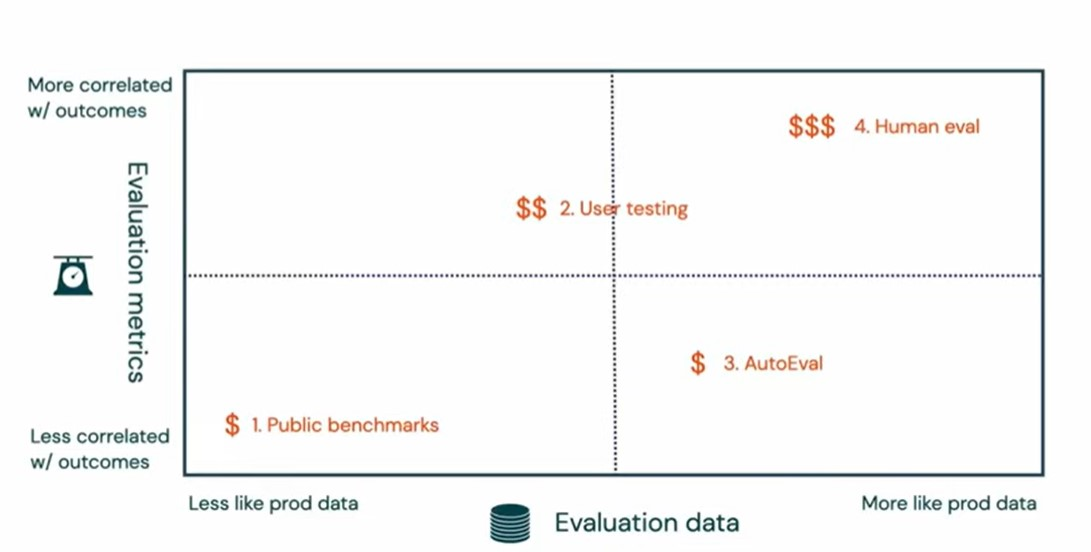
\includegraphics[width=0.8\linewidth,keepaspectratio]{llm69}
\end{center}		


{\tiny (Ref: Evaluating LLM-based Applications // Josh Tobin // LLMs in Prod Conference Part 2 )}

\end{frame}

%%%%%%%%%%%%%%%%%%%%%%%%%%%%%%%%%%%%%%%%%%%%%%%%%%%%%%%%%%%
\begin{frame}[fragile]\frametitle{How to Evaluate}

\begin{itemize}
\item Functional correctness: Code generation models are easy to check
\item Model evaluation models are getting popular.
\item BLUE is getting out of favor due to biases.
\end{itemize}

\begin{center}
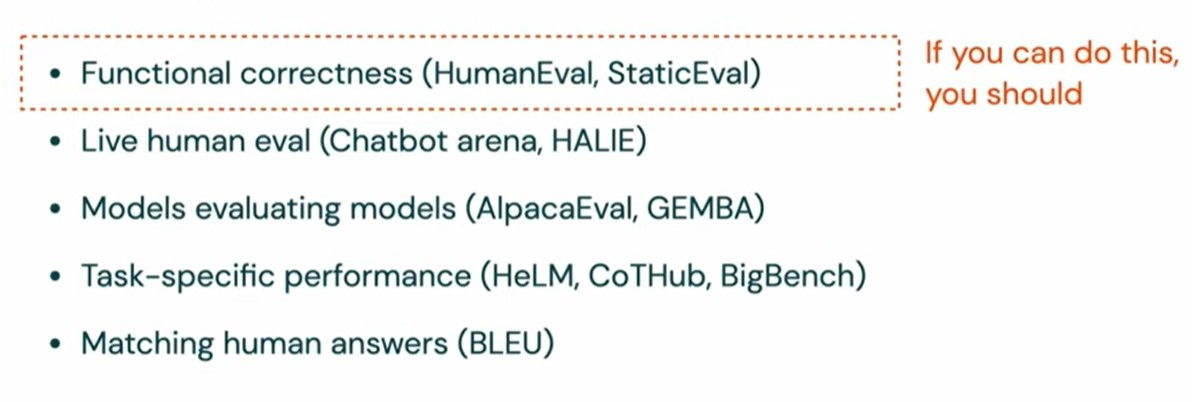
\includegraphics[width=0.8\linewidth,keepaspectratio]{llm70}
\end{center}		


{\tiny (Ref: Evaluating LLM-based Applications // Josh Tobin // LLMs in Prod Conference Part 2 )}

\end{frame}

%%%%%%%%%%%%%%%%%%%%%%%%%%%%%%%%%%%%%%%%%%%%%%%%%%%%%%%%%%%
\begin{frame}[fragile]\frametitle{How to Evaluate}


\begin{center}
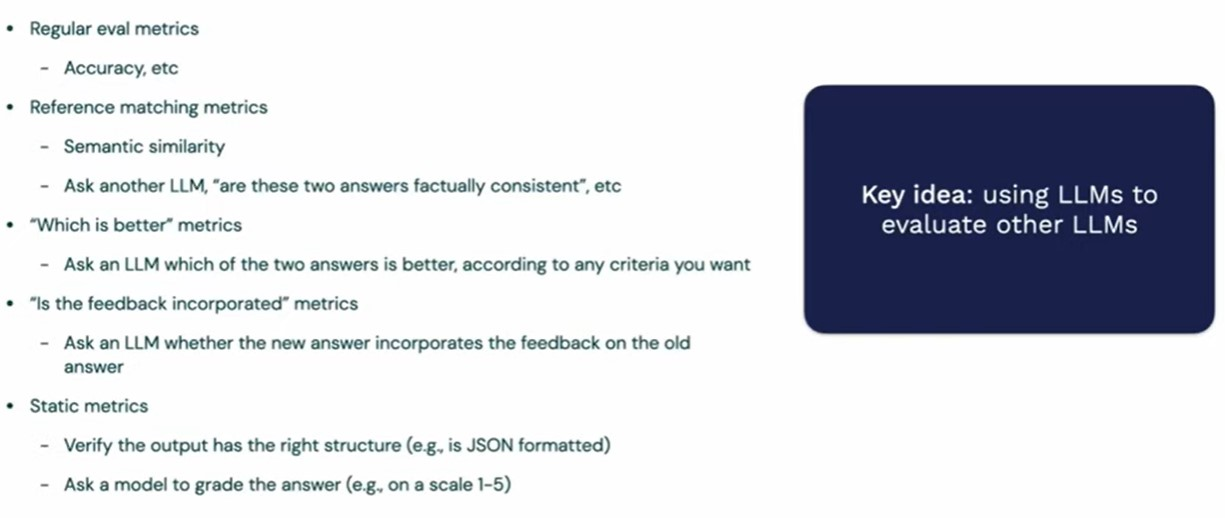
\includegraphics[width=0.8\linewidth,keepaspectratio]{llm71}
\end{center}		

Just note than as LLMs can be biased, using them for evaluation can be limiting. Watching the Watchman!!
Last resort is of course High Quality Human Evaluation.

{\tiny (Ref: Evaluating LLM-based Applications // Josh Tobin // LLMs in Prod Conference Part 2 )}

\end{frame}

%%%%%%%%%%%%%%%%%%%%%%%%%%%%%%%%%%%%%%%%%%%%%%%%%%%%%%%%%%%
\begin{frame}[fragile]\frametitle{How to do costing}

Problem statement: 50\% summarization of whole Wikipedia

\begin{center}
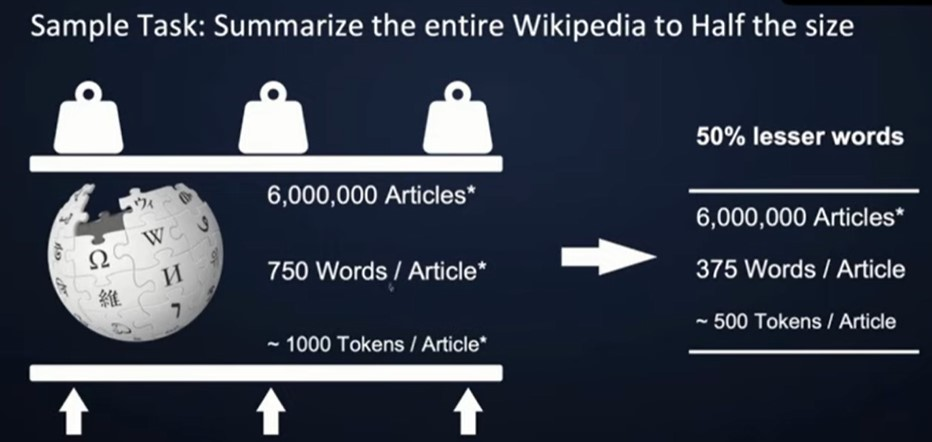
\includegraphics[width=0.8\linewidth,keepaspectratio]{llm72}
\end{center}		



{\tiny (Ref: \$360k Question - Understanding the LLM Economics // Nikunj Bajaj // LLMs in Production Conference )}

\end{frame}

%%%%%%%%%%%%%%%%%%%%%%%%%%%%%%%%%%%%%%%%%%%%%%%%%%%%%%%%%%%
\begin{frame}[fragile]\frametitle{How to do costing}


\begin{center}
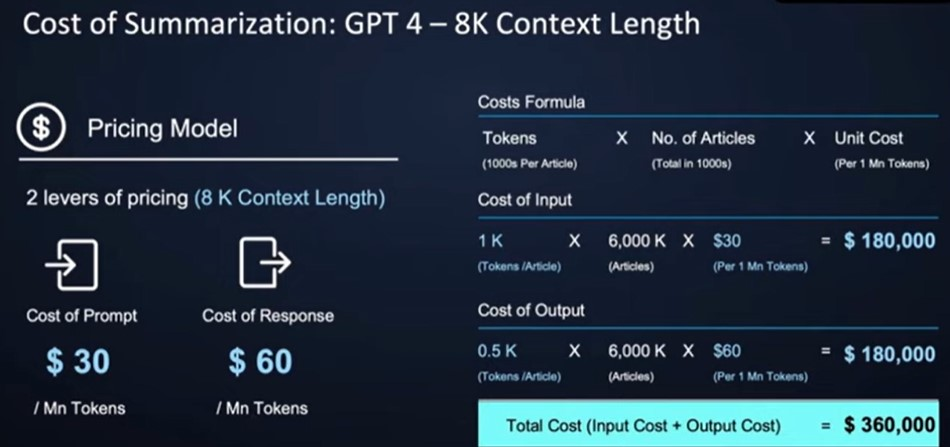
\includegraphics[width=0.8\linewidth,keepaspectratio]{llm73}
\end{center}		



{\tiny (Ref: \$360k Question - Understanding the LLM Economics // Nikunj Bajaj // LLMs in Production Conference )}

\end{frame}

%%%%%%%%%%%%%%%%%%%%%%%%%%%%%%%%%%%%%%%%%%%%%%%%%%%%%%%%%%%
\begin{frame}[fragile]\frametitle{How to do costing}

If we choose bigger context length

\begin{center}
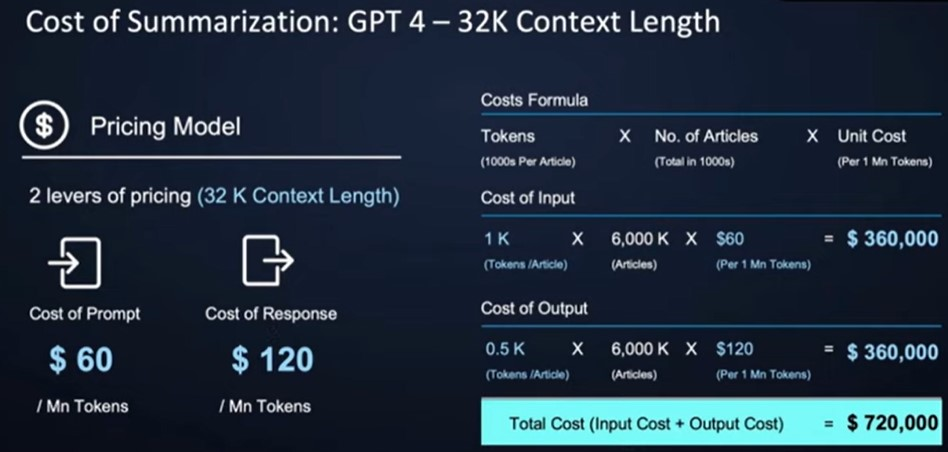
\includegraphics[width=0.8\linewidth,keepaspectratio]{llm74}
\end{center}		



{\tiny (Ref: \$360k Question - Understanding the LLM Economics // Nikunj Bajaj // LLMs in Production Conference )}

\end{frame}

%%%%%%%%%%%%%%%%%%%%%%%%%%%%%%%%%%%%%%%%%%%%%%%%%%%%%%%%%%%
\begin{frame}[fragile]\frametitle{How to do costing}

With Da Vinci

\begin{center}
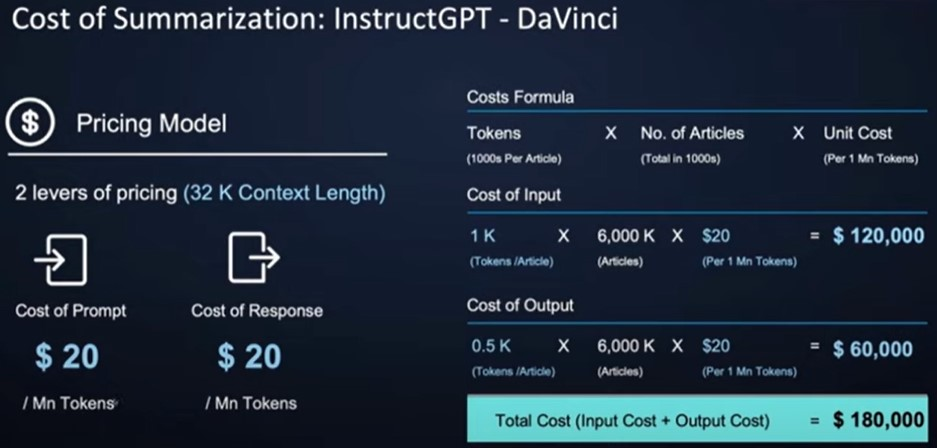
\includegraphics[width=0.8\linewidth,keepaspectratio]{llm75}
\end{center}		



{\tiny (Ref: \$360k Question - Understanding the LLM Economics // Nikunj Bajaj // LLMs in Production Conference )}

\end{frame}

%%%%%%%%%%%%%%%%%%%%%%%%%%%%%%%%%%%%%%%%%%%%%%%%%%%%%%%%%%%
\begin{frame}[fragile]\frametitle{How to do costing}

With Curie

\begin{center}
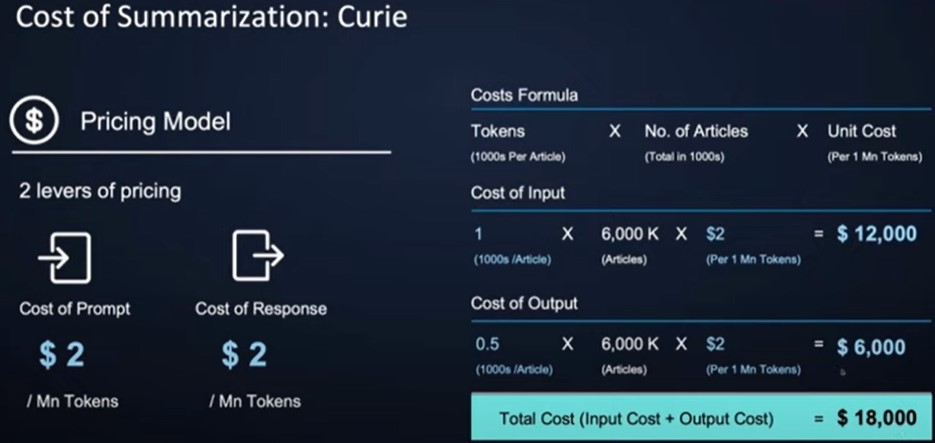
\includegraphics[width=0.8\linewidth,keepaspectratio]{llm76}
\end{center}		



{\tiny (Ref: \$360k Question - Understanding the LLM Economics // Nikunj Bajaj // LLMs in Production Conference )}

\end{frame}

%%%%%%%%%%%%%%%%%%%%%%%%%%%%%%%%%%%%%%%%%%%%%%%%%%%%%%%%%%%
\begin{frame}[fragile]\frametitle{How to do costing}

With self hosted model, speed is assumed to be n tokens per hour

\begin{center}
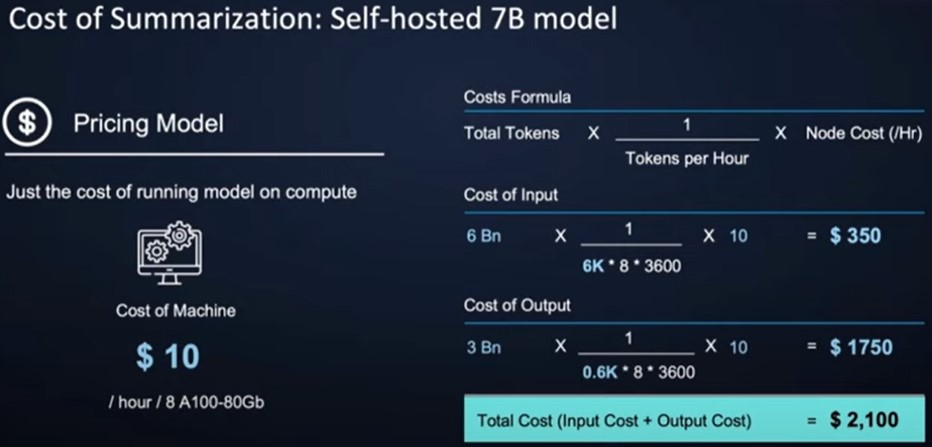
\includegraphics[width=0.8\linewidth,keepaspectratio]{llm77}
\end{center}		



{\tiny (Ref: \$360k Question - Understanding the LLM Economics // Nikunj Bajaj // LLMs in Production Conference )}

\end{frame}

%%%%%%%%%%%%%%%%%%%%%%%%%%%%%%%%%%%%%%%%%%%%%%%%%%%%%%%%%%%
\begin{frame}[fragile]\frametitle{How to do costing}

Fine tuning (Da vinci 1.2M, Curie 126k)
\begin{center}
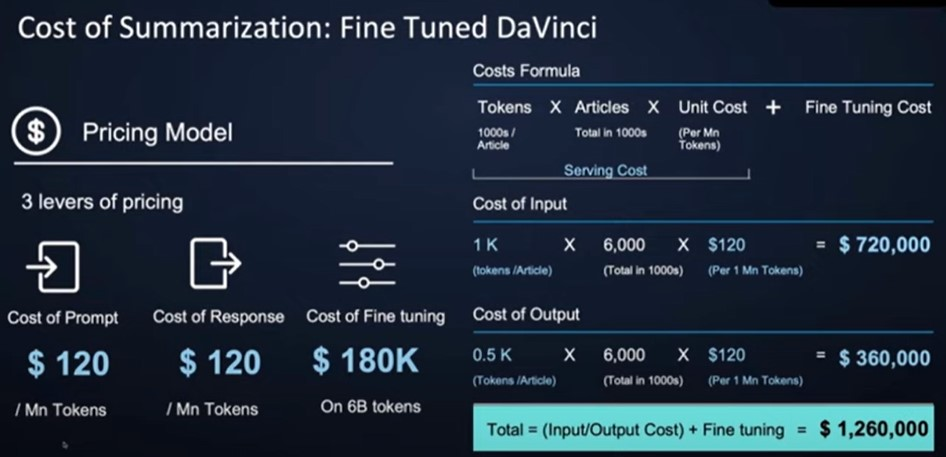
\includegraphics[width=0.8\linewidth,keepaspectratio]{llm78}
\end{center}		



{\tiny (Ref: \$360k Question - Understanding the LLM Economics // Nikunj Bajaj // LLMs in Production Conference )}

\end{frame}

%%%%%%%%%%%%%%%%%%%%%%%%%%%%%%%%%%%%%%%%%%%%%%%%%%%%%%%%%%%
\begin{frame}[fragile]\frametitle{How to do costing}

Fine tuning Self Hosted
\begin{center}
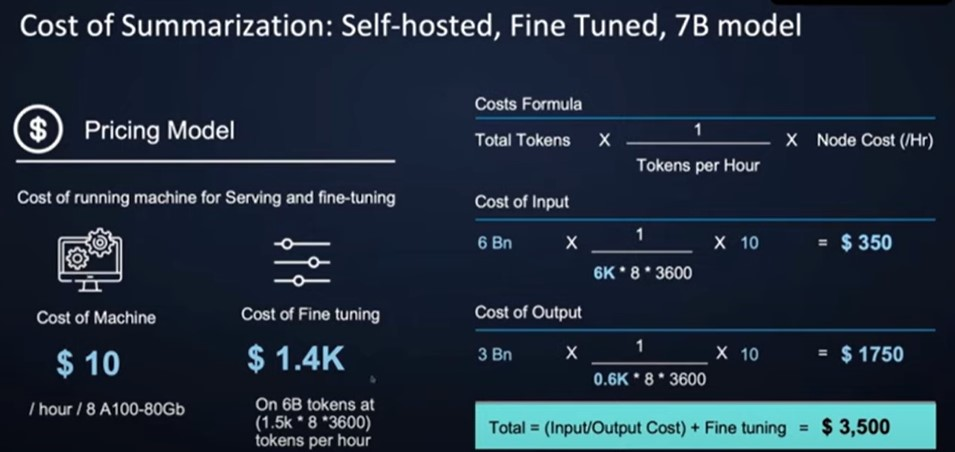
\includegraphics[width=0.8\linewidth,keepaspectratio]{llm79}
\end{center}		



{\tiny (Ref: \$360k Question - Understanding the LLM Economics // Nikunj Bajaj // LLMs in Production Conference )}

\end{frame}

%%%%%%%%%%%%%%%%%%%%%%%%%%%%%%%%%%%%%%%%%%%%%%%%%%%%%%%%%%%
\begin{frame}[fragile]\frametitle{How to do costing}

Summary 

\begin{center}
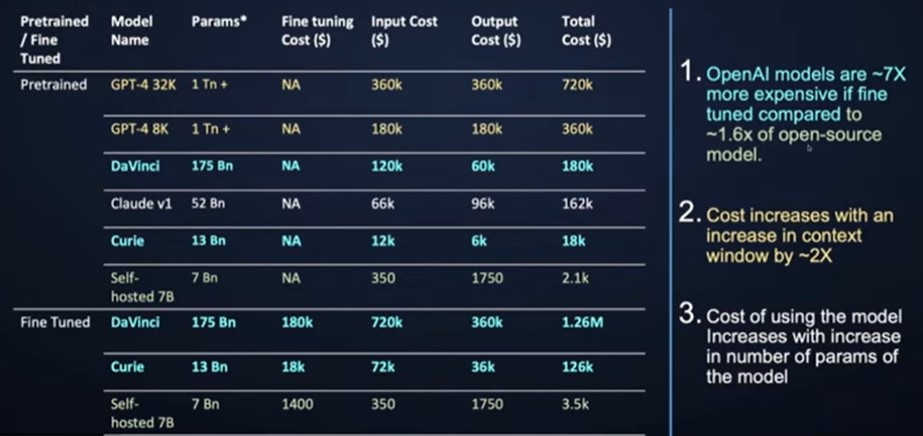
\includegraphics[width=0.8\linewidth,keepaspectratio]{llm80}
\end{center}		



{\tiny (Ref: \$360k Question - Understanding the LLM Economics // Nikunj Bajaj // LLMs in Production Conference )}

\end{frame}

%%%%%%%%%%%%%%%%%%%%%%%%%%%%%%%%%%%%%%%%%%%%%%%%%%%%%%%%%%%
\begin{frame}[fragile]\frametitle{How to do costing}

Summary with quality also

\begin{center}
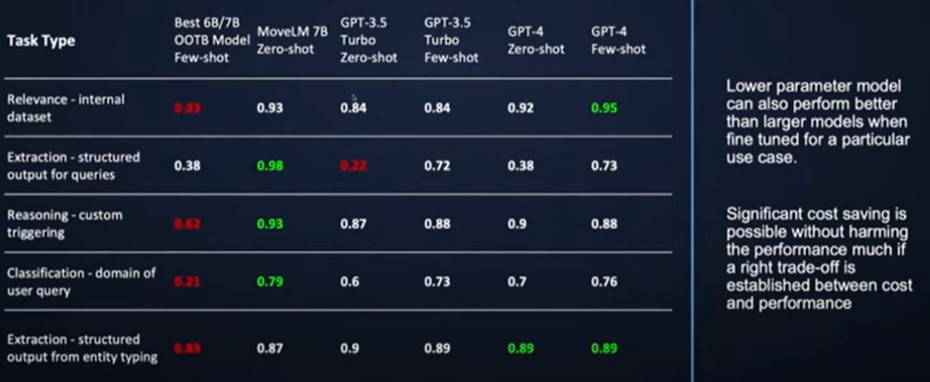
\includegraphics[width=0.8\linewidth,keepaspectratio]{llm81}
\end{center}		

Open source LLM with fine tuning is the recommendation.


{\tiny (Ref: \$360k Question - Understanding the LLM Economics // Nikunj Bajaj // LLMs in Production Conference )}

\end{frame}




%%%%%%%%%%%%%%%%%%%%%%%%%%%%%%%%%%%%%%%%%%%%%%%%%%%%%%%%%%%
\begin{frame}[fragile]\frametitle{Shared Responsibility Model}

\begin{center}
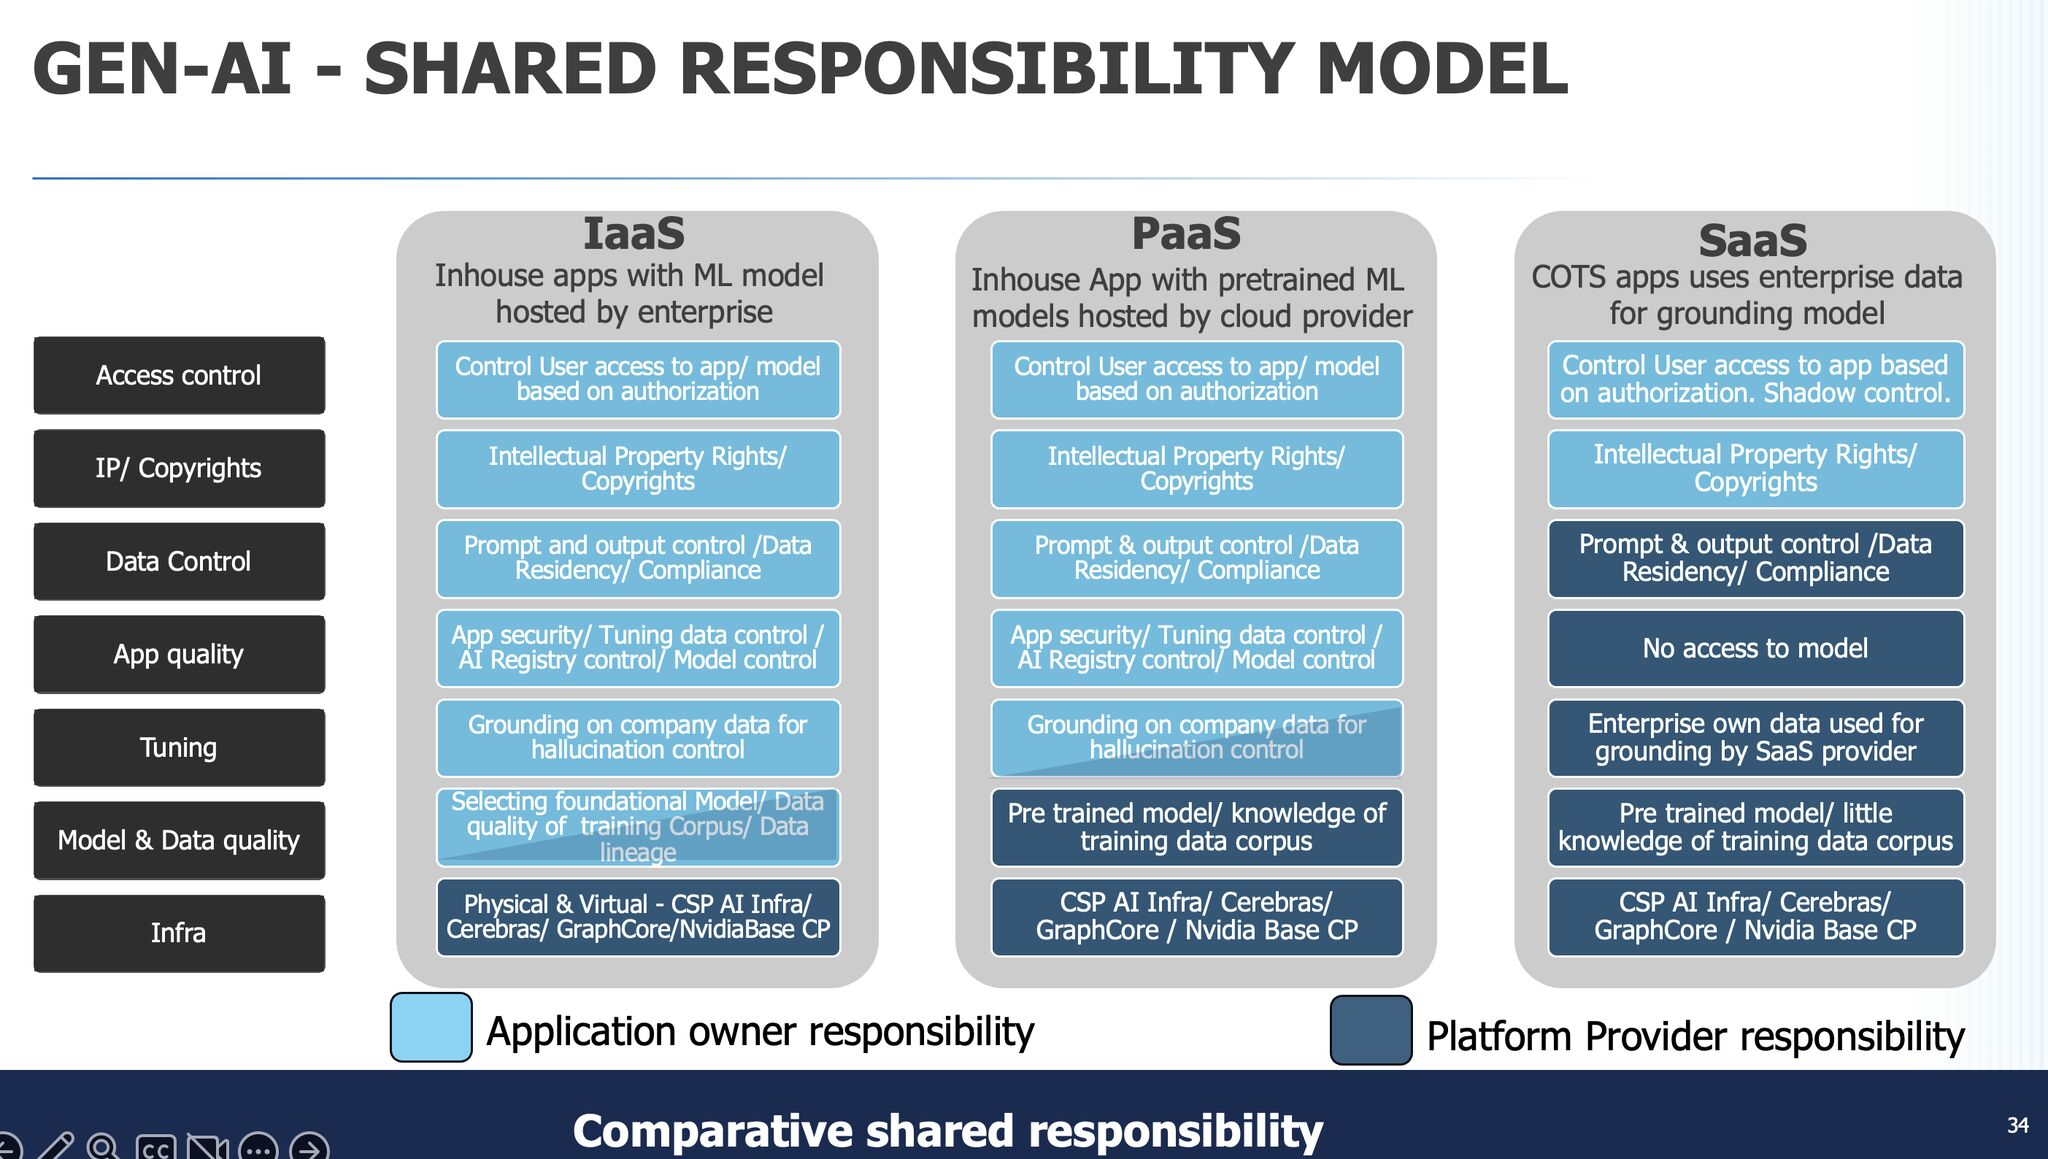
\includegraphics[width=\linewidth,keepaspectratio]{llm63}
\end{center}		


{\tiny (Ref: Linkedin Post on 11 Aug 2023 by - Vishwas Manral )}

\end{frame}


%%%%%%%%%%%%%%%%%%%%%%%%%%%%%%%%%%%%%%%%%%%%%%%%%%%%%%%%%%%
\begin{frame}[fragile]\frametitle{Commercial Example: Intuit GenOS}

\begin{itemize}
    \item GenStudio: Dev environment for rapid experimentation with generative AI experiences.
    \item GenRuntime: Intelligent layer choosing appropriate large language model in real time, based on user needs.
    \item GenUX: Library of UI components and user flows for clear and delightful interactions.
    \item Financial LLMs: Custom trained for tax, accounting, marketing, etc., providing insights and actions.
\end{itemize}

\end{frame}

%%%%%%%%%%%%%%%%%%%%%%%%%%%%%%%%%%%%%%%%%%%%%%%%%%%%%%%%%%%%%%%%%%%%%%%%%%%%%%%%%%
\begin{frame}[fragile]\frametitle{Challenges of Building LLM App}


\begin{center}
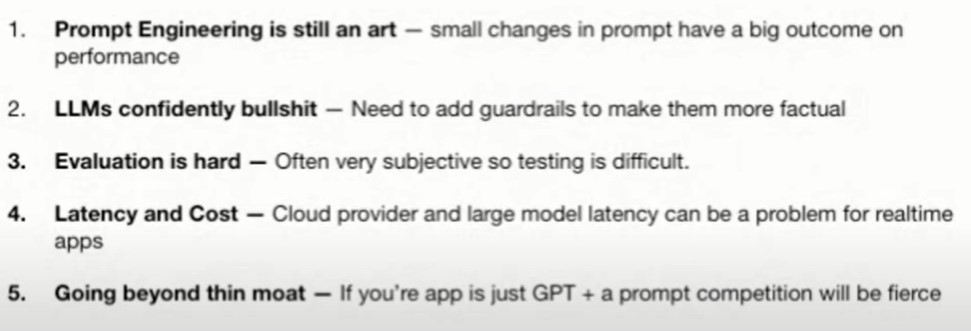
\includegraphics[width=0.7\linewidth,keepaspectratio]{llm83}

\end{center}

{\tiny (Ref: Pitfalls and Best Practices — 5 lessons from LLMs in Production // Raza Habib // LLMs in Prod Con 2)}
\end{frame}

%%%%%%%%%%%%%%%%%%%%%%%%%%%%%%%%%%%%%%%%%%%%%%%%%%%%%%%%%%%%%%%%%%%%%%%%%%%%%%%%%%
\begin{frame}[fragile]\frametitle{Challenges of Building LLM App}


\begin{center}
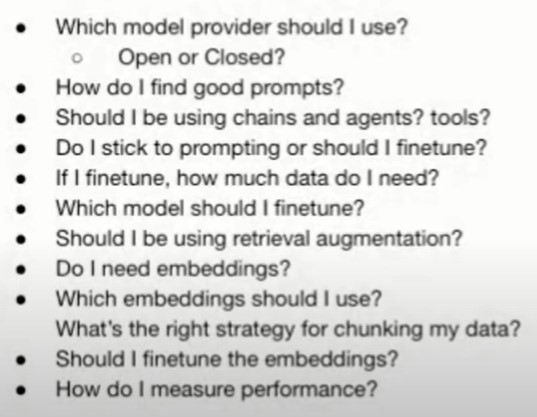
\includegraphics[width=0.7\linewidth,keepaspectratio]{llm84}

\end{center}

{\tiny (Ref: Pitfalls and Best Practices — 5 lessons from LLMs in Production // Raza Habib // LLMs in Prod Con 2)}
\end{frame}


%%%%%%%%%%%%%%%%%%%%%%%%%%%%%%%%%%%%%%%%%%%%%%%%%%%%%%%%%%%%%%%%%%%%%%%%%%%%%%%%%%
\begin{frame}[fragile]\frametitle{}
\begin{center}
{\Large Design Patterns in Production}

{\tiny (Ref: Using Vector Databases: Practical Advice for Production // Sam Partee // LLMs in Prod Conference)}

\end{center}
\end{frame}

%%%%%%%%%%%%%%%%%%%%%%%%%%%%%%%%%%%%%%%%%%%%%%%%%%%%%%%%%%%%%%%%%%%%%%%%%%%%%%%%%%
\begin{frame}[fragile]\frametitle{Context}


\begin{center}
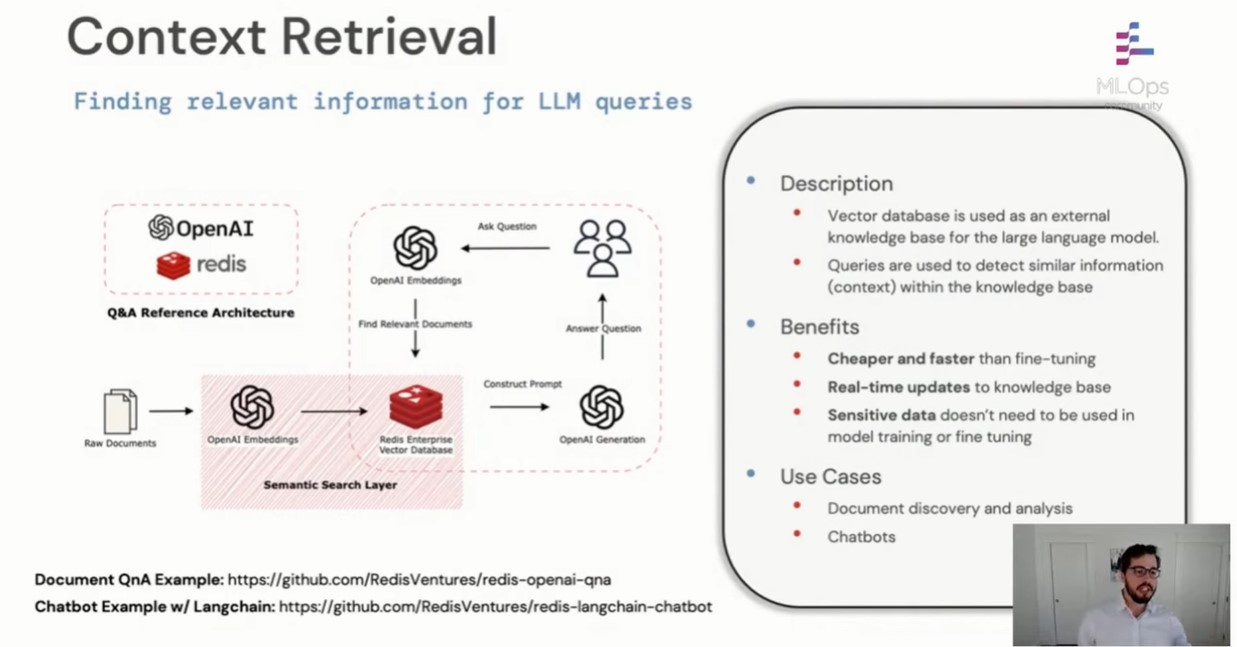
\includegraphics[width=\linewidth,keepaspectratio]{llm92}

\end{center}

Ideal for rapidly changing knowledge base, no need to change LLM. Also, good for local/private data.

\end{frame}

%%%%%%%%%%%%%%%%%%%%%%%%%%%%%%%%%%%%%%%%%%%%%%%%%%%%%%%%%%%%%%%%%%%%%%%%%%%%%%%%%%
\begin{frame}[fragile]\frametitle{Hype}


\begin{center}
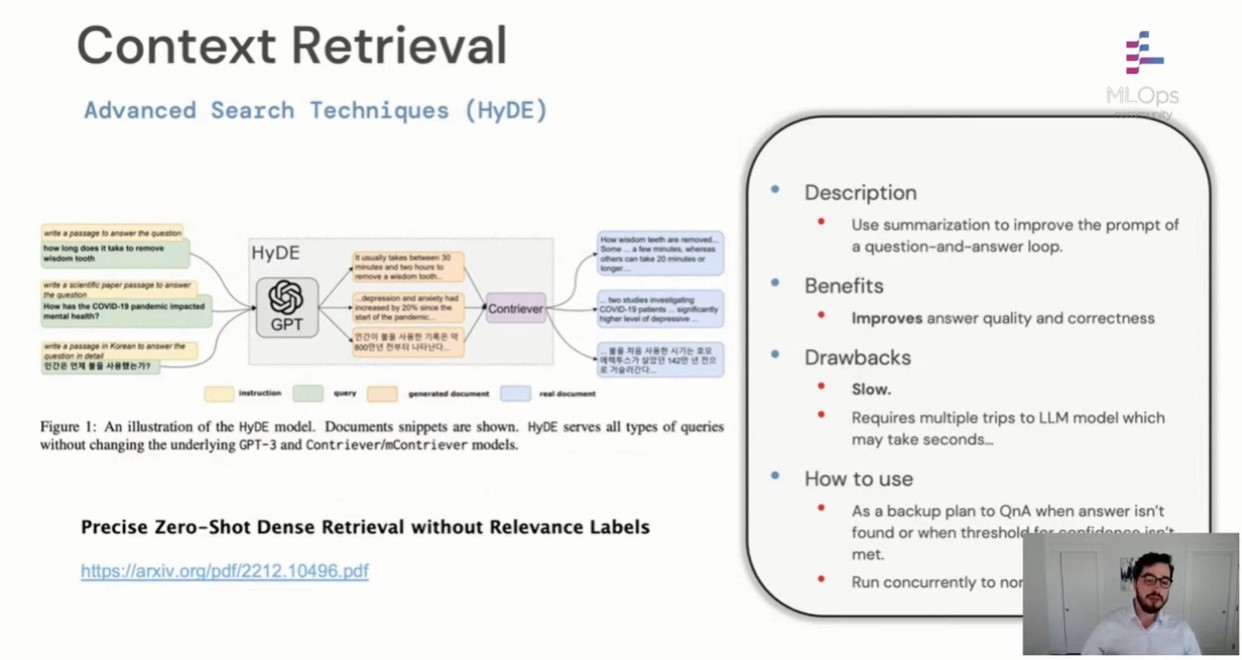
\includegraphics[width=\linewidth,keepaspectratio]{llm93}

\end{center}

Two call, summurization on top of retrieval.
\end{frame}

%%%%%%%%%%%%%%%%%%%%%%%%%%%%%%%%%%%%%%%%%%%%%%%%%%%%%%%%%%%%%%%%%%%%%%%%%%%%%%%%%%
\begin{frame}[fragile]\frametitle{Features}


\begin{center}
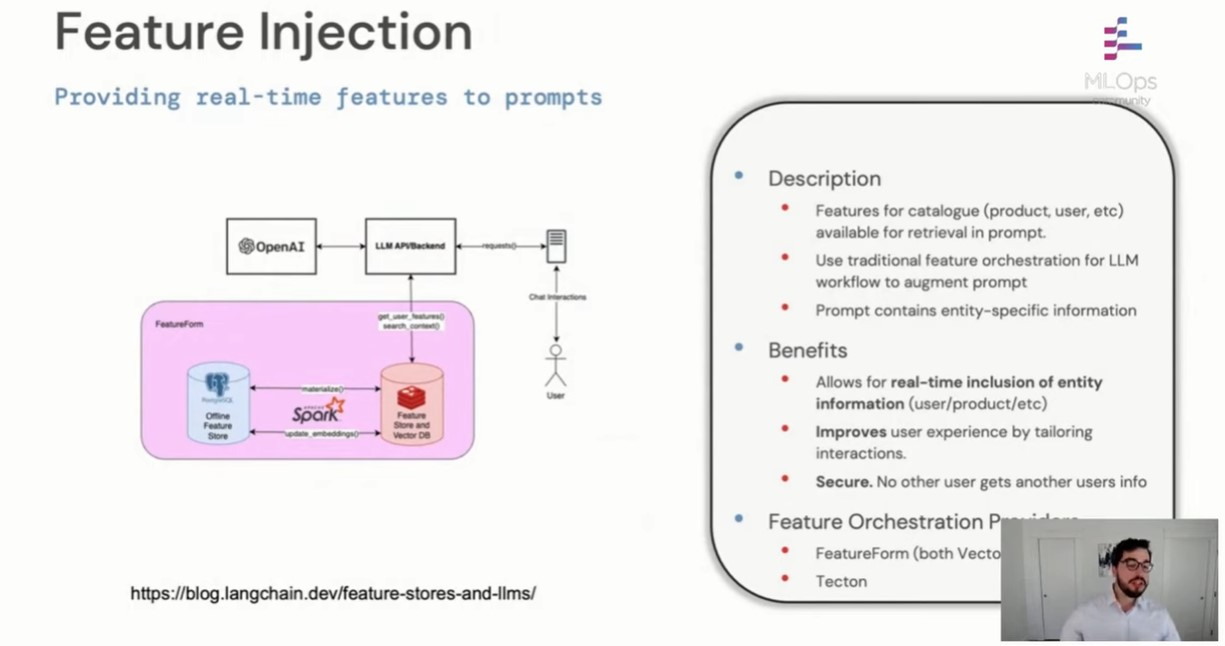
\includegraphics[width=\linewidth,keepaspectratio]{llm94}

\end{center}

Context + features
\end{frame}

%%%%%%%%%%%%%%%%%%%%%%%%%%%%%%%%%%%%%%%%%%%%%%%%%%%%%%%%%%%%%%%%%%%%%%%%%%%%%%%%%%
\begin{frame}[fragile]\frametitle{Caching}


\begin{center}
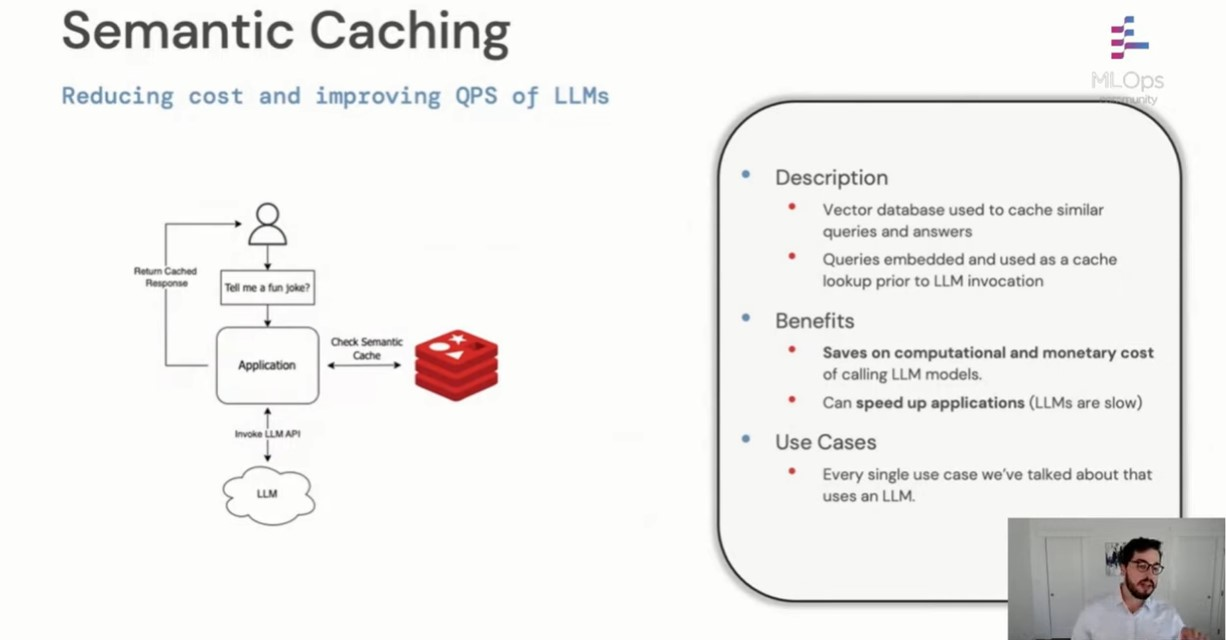
\includegraphics[width=\linewidth,keepaspectratio]{llm95}

\end{center}

Caching popular contexts
\end{frame}

%%%%%%%%%%%%%%%%%%%%%%%%%%%%%%%%%%%%%%%%%%%%%%%%%%%%%%%%%%%%%%%%%%%%%%%%%%%%%%%%%%
\begin{frame}[fragile]\frametitle{Guardrails}


\begin{center}
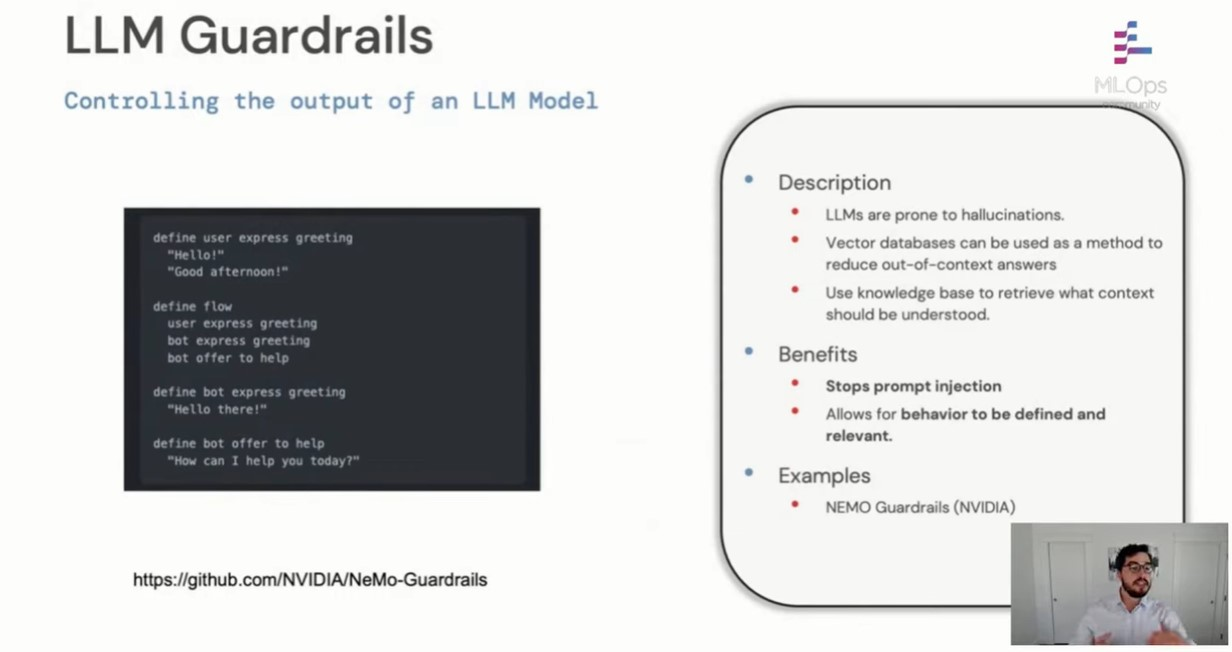
\includegraphics[width=\linewidth,keepaspectratio]{llm96}

\end{center}

Post processing
\end{frame}

%%%%%%%%%%%%%%%%%%%%%%%%%%%%%%%%%%%%%%%%%%%%%%%%%%%%%%%%%%%%%%%%%%%%%%%%%%%%%%%%%%
\begin{frame}[fragile]\frametitle{Memory}


\begin{center}
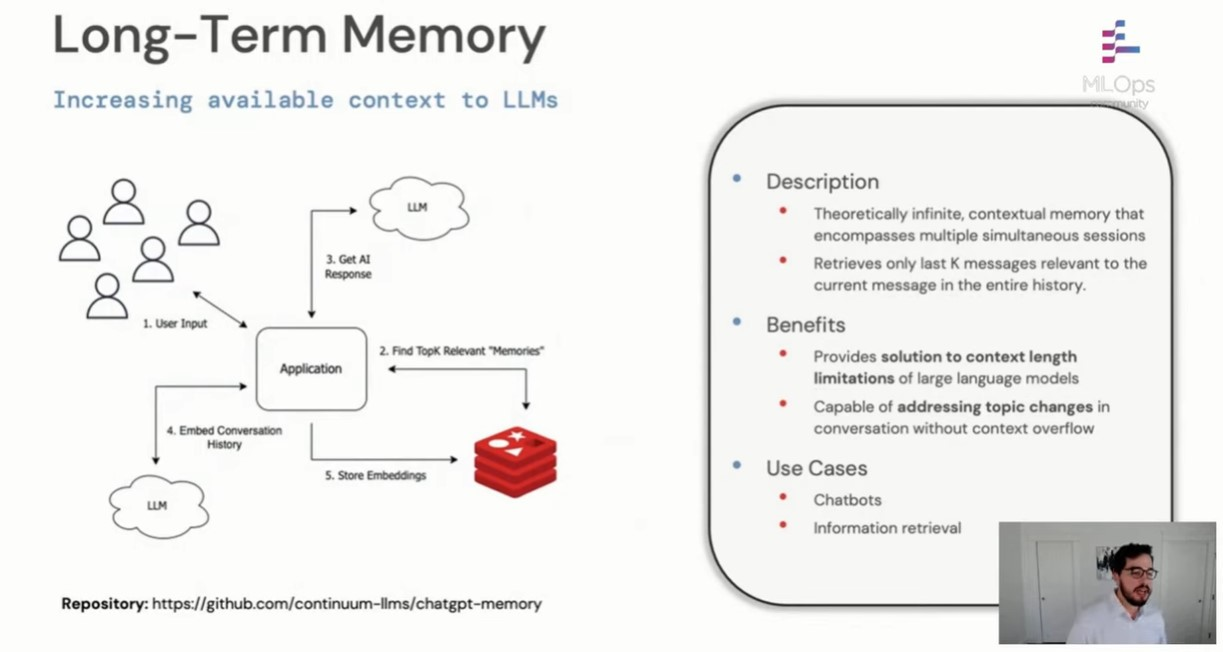
\includegraphics[width=\linewidth,keepaspectratio]{llm97}

\end{center}

Keep History
\end{frame}

%%%%%%%%%%%%%%%%%%%%%%%%%%%%%%%%%%%%%%%%%%%%%%%%%%%%%%%%%%%%%%%%%%%%%%%%%%%%%%%%%%
\begin{frame}[fragile]\frametitle{Mistakes}


\begin{center}
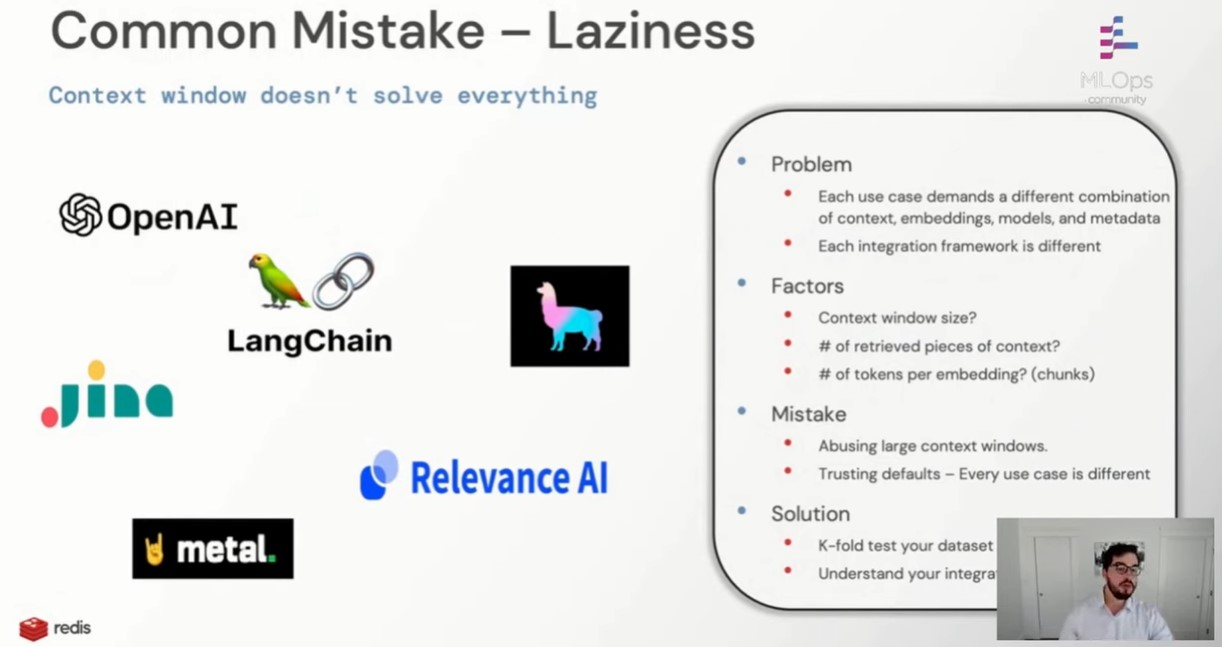
\includegraphics[width=\linewidth,keepaspectratio]{llm98}

\end{center}

\end{frame}

%%%%%%%%%%%%%%%%%%%%%%%%%%%%%%%%%%%%%%%%%%%%%%%%%%%%%%%%%%%
\begin{frame}[fragile]\frametitle{Project LifeCycle}


		\begin{center}
		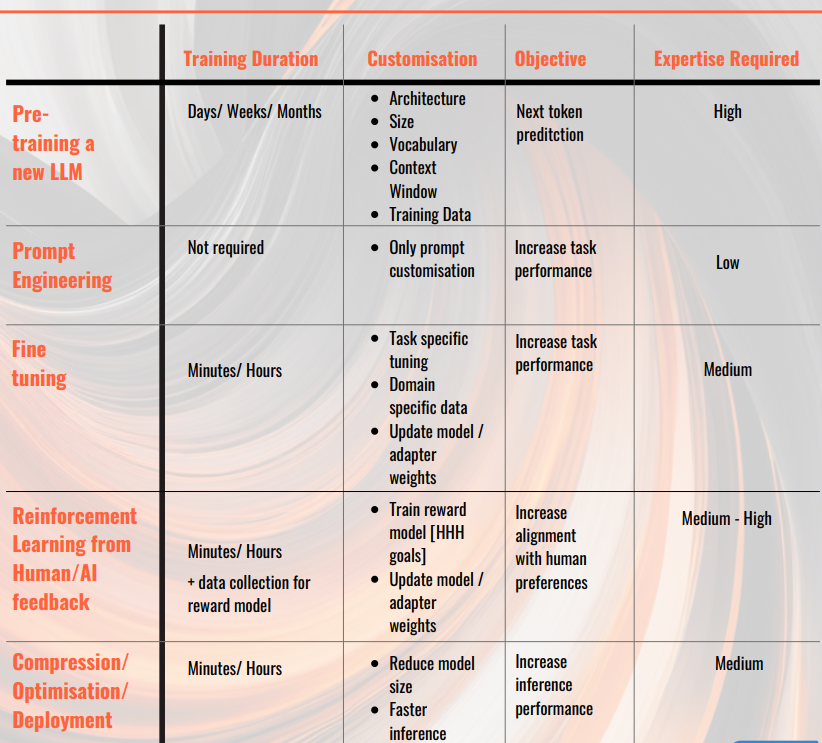
\includegraphics[width=0.6\linewidth,keepaspectratio]{rag5}
		\end{center}

{\tiny (Ref: RAG Architecture -Abhinav  Kimothi)}

\end{frame}

%%%%%%%%%%%%%%%%%%%%%%%%%%%%%%%%%%%%%%%%%%%%%%%%%%%%%%%%%%%%%%%%%%%%%%%%%%%%%%%%%%
\begin{frame}[fragile]\frametitle{}
\begin{center}
{\Large  LLMOps}

{\tiny (Ref: Evolving LLMOps Stack for RAG - Abhinav Kimothi)}

\end{center}
\end{frame}

%%%%%%%%%%%%%%%%%%%%%%%%%%%%%%%%%%%%%%%%%%%%%%%%%%%%%%%%%%%
\begin{frame}[fragile]\frametitle{Evolving LLMOps Stack for RAG}


		\begin{center}
		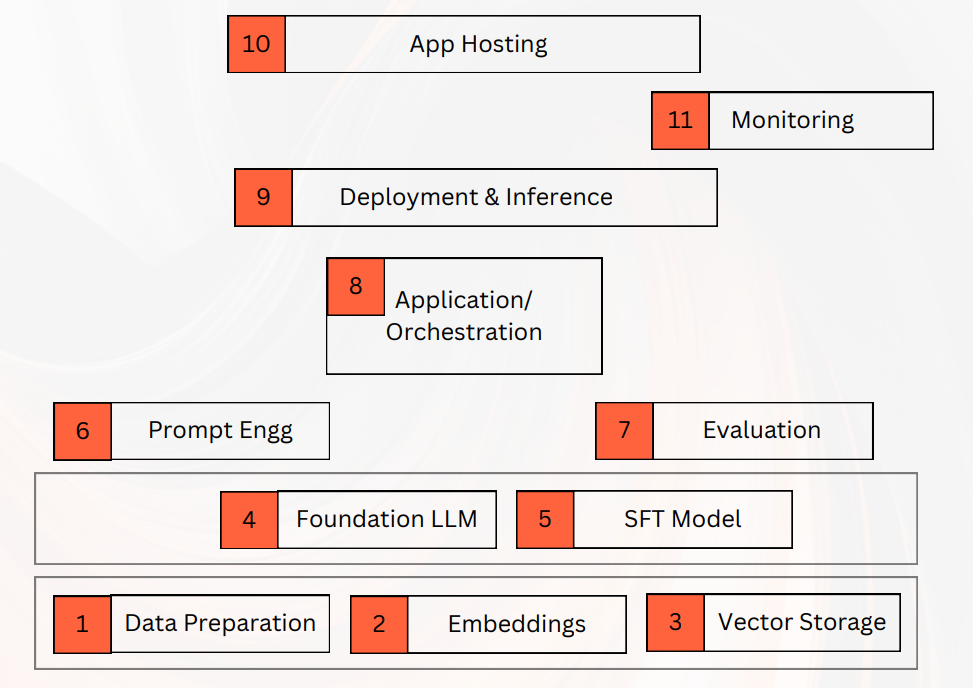
\includegraphics[width=0.6\linewidth,keepaspectratio]{rag25}
		\end{center}

{\tiny (Ref: RAG Architecture -Abhinav  Kimothi)}

\end{frame}

%%%%%%%%%%%%%%%%%%%%%%%%%%%%%%%%%%%%%%%%%%%%%%%%%%%%%%%%%%%
\begin{frame}[fragile]\frametitle{Data Layer}
    \begin{itemize}
        \item Data preparation involves Sourcing, Cleaning, Loading \& Chunking.
        \item Creation of Embeddings is a crucial step in the data layer.
        \item Storing embeddings in a vector store is essential for retrieval.
    \end{itemize}
	
	\begin{center}
	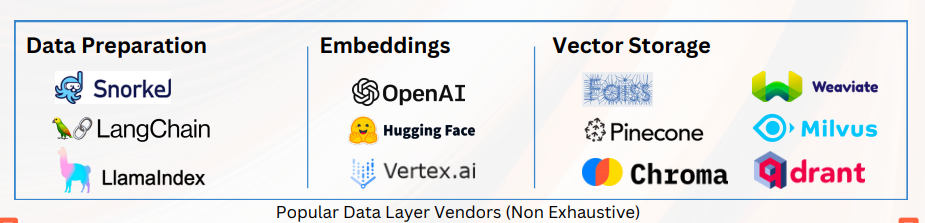
\includegraphics[width=0.6\linewidth,keepaspectratio]{rag26}
	
	{\tiny (Ref: RAG Architecture -Abhinav  Kimothi)}
	\end{center}
		
\end{frame}

%%%%%%%%%%%%%%%%%%%%%%%%%%%%%%%%%%%%%%%%%%%%%%%%%%%%%%%%%%%
\begin{frame}[fragile]\frametitle{Model Layer}
    \begin{itemize}
        \item Four categories of LLMs in RAG applications: Proprietary, Open Source, Supervised Fine-Tuned Proprietary, Supervised Fine-Tuned Open Source.
        \item Providers like OpenAI, Anthropic, and Google offer Proprietary Foundation Models.
        \item Open Source Foundation Models (e.g., Falcon, Llama, Mistral) require hosting and maintenance by users.
        \item Fine-tuning options available for both Proprietary and Open Source models.
        \item Vendors facilitate access to open source models and support easy fine-tuning.
    \end{itemize}
	
	\begin{center}
	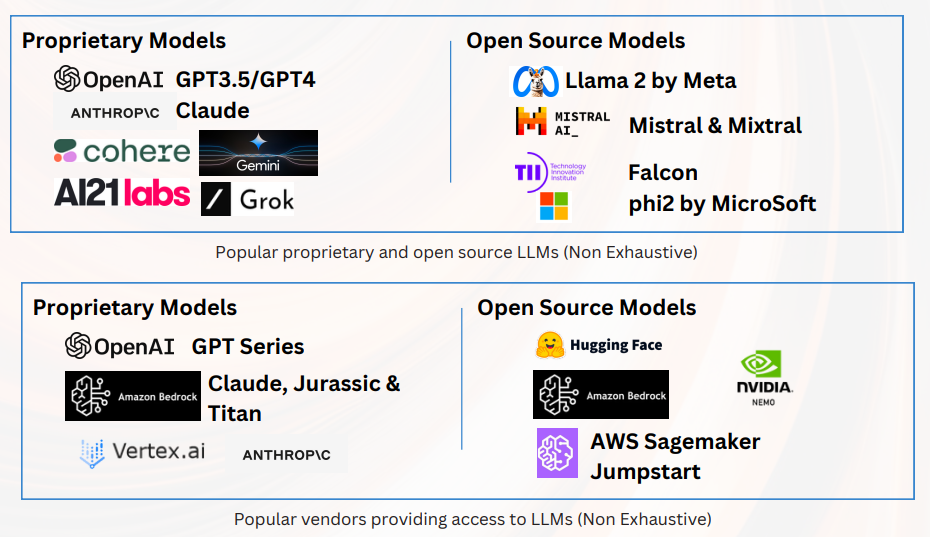
\includegraphics[width=0.6\linewidth,keepaspectratio]{rag27}
	
	{\tiny (Ref: RAG Architecture -Abhinav  Kimothi)}
	\end{center}	
\end{frame}

%%%%%%%%%%%%%%%%%%%%%%%%%%%%%%%%%%%%%%%%%%%%%%%%%%%%%%%%%%%
\begin{frame}[fragile]\frametitle{Prompt Layer}
    \begin{itemize}
        \item Prompt Engineering goes beyond natural language questions.
        \item Developers employ various techniques and iterate on prompts for effectiveness.
        \item Experimentation is crucial in creating tailored prompts for specific use cases.
        \item The process requires tracking and collaboration among developers.
    \end{itemize}
	
	\begin{center}
	
\includegraphics[width=0.6\linewidth,keepaspectratio]{rag28}
	
	{\tiny (Ref: RAG Architecture -Abhinav  Kimothi)}
	\end{center}		
\end{frame}

%%%%%%%%%%%%%%%%%%%%%%%%%%%%%%%%%%%%%%%%%%%%%%%%%%%%%%%%%%%
\begin{frame}[fragile]\frametitle{Evaluation}
    \begin{itemize}
        \item Building a RAG pipeline is one thing; robust evaluation is crucial for production readiness.
        \item Frameworks and tools available for evaluating hallucinations, relevance, and accuracy.
    \end{itemize}
	
	\begin{center}
	
\includegraphics[width=0.6\linewidth,keepaspectratio]{rag29}
	
	{\tiny (Ref: RAG Architecture -Abhinav  Kimothi)}
	\end{center}			
\end{frame}

%%%%%%%%%%%%%%%%%%%%%%%%%%%%%%%%%%%%%%%%%%%%%%%%%%%%%%%%%%%
\begin{frame}[fragile]\frametitle{App Orchestration}
    \begin{itemize}
        \item RAG application involves multiple tools and services.
        \item Solid orchestration framework needed to invoke different processes in the pipeline.
    \end{itemize}
	
	\begin{center}
	
\includegraphics[width=0.6\linewidth,keepaspectratio]{rag30}
	
	{\tiny (Ref: RAG Architecture -Abhinav  Kimothi)}
	\end{center}		
\end{frame}

%%%%%%%%%%%%%%%%%%%%%%%%%%%%%%%%%%%%%%%%%%%%%%%%%%%%%%%%%%%
\begin{frame}[fragile]\frametitle{Deployment Layer}
    \begin{itemize}
        \item Deployment on various cloud providers and platforms is possible.
        \item Considerations include Security, Governance, Logging, Inference costs, and latency.
    \end{itemize}
	
	\begin{center}
	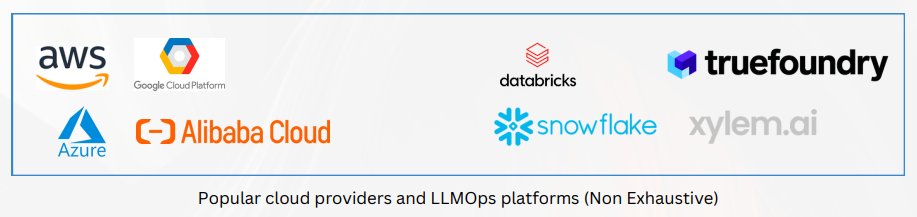
\includegraphics[width=0.6\linewidth,keepaspectratio]{rag31}
	
	{\tiny (Ref: RAG Architecture -Abhinav  Kimothi)}
	\end{center}
	
\end{frame}

%%%%%%%%%%%%%%%%%%%%%%%%%%%%%%%%%%%%%%%%%%%%%%%%%%%%%%%%%%%
\begin{frame}[fragile]\frametitle{Application Layer}
    \begin{itemize}
        \item Application needs to be hosted for users or systems to interact with.
        \item Options include creating a custom application layer or using available platforms.
    \end{itemize}
	
	\begin{center}
	
\includegraphics[width=0.6\linewidth,keepaspectratio]{rag32}
	
	{\tiny (Ref: RAG Architecture -Abhinav  Kimothi)}
	\end{center}
	
\end{frame}

%%%%%%%%%%%%%%%%%%%%%%%%%%%%%%%%%%%%%%%%%%%%%%%%%%%%%%%%%%%
\begin{frame}[fragile]\frametitle{Monitoring}
    \begin{itemize}
        \item Continuous monitoring of deployed application for accuracy, relevance, cost, and latency.
    \end{itemize}
	
	\begin{center}
	
\includegraphics[width=0.6\linewidth,keepaspectratio]{rag33}
	
	{\tiny (Ref: RAG Architecture -Abhinav  Kimothi)}
	\end{center}	
\end{frame}

%%%%%%%%%%%%%%%%%%%%%%%%%%%%%%%%%%%%%%%%%%%%%%%%%%%%%%%%%%%
\begin{frame}[fragile]\frametitle{Other Considerations}
    \begin{itemize}
        \item LLM Cache: Reduce costs by saving responses for popular queries.
        \item LLM Guardrails: Add an additional layer of scrutiny on generations.
    \end{itemize}
\end{frame}

